\documentclass[12pt]{article}

\usepackage[utf8]{inputenc}
\usepackage[T1]{fontenc}
\usepackage[ngerman]{babel}
\usepackage[ngerman=ngerman-x-latest]{hyphsubst}
\usepackage{csquotes}
\usepackage{hyphenat}
\usepackage{textcmds}
\usepackage{xspace}
\usepackage{listings}
\usepackage{amsmath}
\usepackage{amsfonts}
\usepackage{mathtools}

\usepackage{authblk}
\renewcommand*{\Authsep}{, }
\renewcommand*{\Authand}{ und }
\renewcommand*{\Authands}{ und }

\usepackage{geometry}
\geometry{a4paper, margin=1in}

\usepackage{graphicx}
\usepackage{chngpage}
\usepackage{calc}

\renewcommand{\lstlistingname}{Code}
\renewcommand{\lstlistlistingname}{Codeverzeichnis}

\usepackage{hyperref}
\hypersetup{
    colorlinks=true,
    linkcolor=black,
    filecolor=blue,
    urlcolor=blue,
    pdftitle={Semesterprojekt},
    pdfauthor={Nik Benson},
    pdfpagemode=FullScreen,
}
\urlstyle{same}

\usepackage{pgfplots}
\usepackage{pgfplotstable}

\usepackage{booktabs}
\usepackage{siunitx}
\usepackage{csvsimple}

\usepgfplotslibrary{units}

\usepackage{xcolor}
\definecolor{codegreen}{rgb}{0,0.6,0}
\definecolor{codegray}{rgb}{0.5,0.5,0.5}
\definecolor{codepurple}{rgb}{0.58,0,0.82}
\definecolor{backcolour}{rgb}{0.95,0.95,0.92}

\lstdefinestyle{c}{
    backgroundcolor=\color{backcolour},
    commentstyle=\color{codegreen},
    keywordstyle=\color{magenta},
    numberstyle=\tiny\color{codegray},
    stringstyle=\color{codepurple},
    basicstyle=\ttfamily\footnotesize,
    breakatwhitespace=false,
    breaklines=true,
    captionpos=b,
    keepspaces=true,
    numbers=left,
    numbersep=5pt,
    showspaces=false,
    showstringspaces=false,
    showtabs=false,
    tabsize=2
}

\lstset{style=c}

\DeclarePairedDelimiter\ceil{\lceil}{\rceil}
\DeclarePairedDelimiter\floor{\lfloor}{\rfloor}

\title{Semesterprojekt}
\author[1]{Nik Benson}
\affil[1]{\href{mailto:nik.benson@studmail.w-hs.de}{nik.benson@studmail.w-hs.de}}
\author[2]{<name>}
\affil[2]{\href{mailto:<email>}{<email>}}
\author[3]{<name>}
\affil[3]{\href{mailto:<email>}{<email>}}
\author[4]{<name>}
\affil[4]{\href{mailto:<email>}{<email>}}

\begin{document}
    \pagenumbering{gobble}
    \begin{titlepage}
    \maketitle
    \vspace{3cm}
    \begin{tabular}{l c r}
        
\includegraphics[width={0.45\textwidth}]{../assets/img/whs}
        & \hspace*{\fill} &
        \includesvg[width=0.45\textwidth]{../assets/img/netTrek}
    \end{tabular}
    \vspace*{\fill}
    \begin{flushleft}
        \Large{\textbf{Institution:} Westfälische Hochschule}\\
        \Large{\textbf{Modul:} \href{https://moodle.w-hs.de/course/view.php?id=36}{Student's Lab}} \\
        \Large{\textbf{Prüfer:} Prof. Dr. Martin Guddat}\\
        \Large{\textbf{Semester:} WiSe 22/23}
    \end{flushleft}
\end{titlepage}


    \pagenumbering{Roman}
    \addcontentsline{toc}{section}{Inhaltsverzeichnis}
    \tableofcontents
    \newpage
    \addcontentsline{toc}{section}{Abbildungsverzeichnis}
    \listoffigures
    \addcontentsline{toc}{section}{Codeverzeichnis}
    \lstlistoflistings
    \newpage
    \pagenumbering{arabic}


    \section{Ziele}

        \subsection{MVP}
            \begin{enumerate}
                \item Labyrinth wird generiert mit Java
                \item Labyrinth wird in top down ansicht dargestellt mit Processing
            \end{enumerate}

        \subsection{Milestones}
            \begin{enumerate}
                \item Bewegen durch das Labyrinth
                \item First Person
                \item Varianten bei der Generierung
                \item Level Editor
                \item P5JS
                \item Ball
            \end{enumerate}

    \section{Generieren eines rechteckigen Labyrinths}\label{sec:generieren-eines-rechteckigen-labyrinths}
        Wir haben uns für den \qq{Randomised-Depth-First-Search} Algorithmus entschieden.
        \subsection{Randomized-Depth-First-Search}\label{subsec:randomized-depth-first-search}
            \begin{figure}
                \centering
                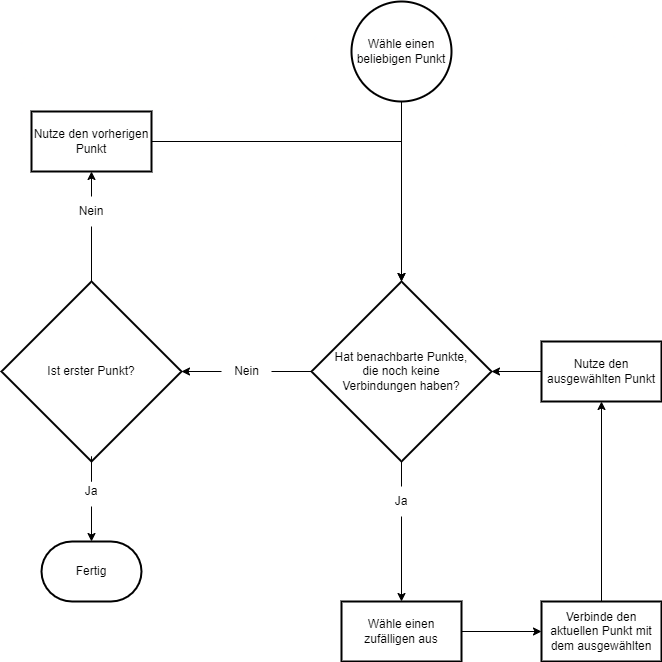
\includegraphics[width=\paperwidth/2]{../assets/img/Randomised-Depth-First-Search}
                \caption{Randomized-Depth-First-Search Ablauf}
                \label{fig:randomized-depth-first-search-flow}
            \end{figure}
            Gegeben ist ein Feld der Breite $w$ und Höhe $h$.
            Das Feld beinhaltet alle Punkte $p\in\{(x,y)\in\mathbb{N}^2, 0\leq x<w, 0\leq y<h\}$.
            Daraus wird zunächst ein beliebiger Startpunkt ausgewählt.
            Die benachbarten Punkte werden nach Punkten durchsucht, die noch keine Verbindungen haben.
            Der Startpunkt wird zufällig mit einem dieser Punkte verbunden.
            Anschließend wird der verbindungspunkt zum neuen Startpunkt.
            Hat der Startpunkt keine benachbarten Punkte ohne Verbindungen, so wird der vorherige Startpunkt überprüft.
            Dies wird wiederholt, bis es keinen Punkt mehr gibt, der keine Verbindung hat.
            Der Ablauf ist auch in Abbildung~\ref{fig:randomized-depth-first-search-flow} dargestellt.

        \subsection{Unsere Implementierung}\label{subsec:unsere-implementierung}
            \begin{lstlisting}[label={lst:randomised-depth-first-search-code}, caption={Randomized-Depth-First-Search Implementierung}]
private void recursivePathGeneration(Coordinate current) {
    for (Coordinate[] adjacent = generateCandidates(current); adjacent.length != 0; adjacent = generateCandidates(current)) {
        Coordinate next = adjacent[random.nextInt(adjacent.length)];

        graph.addEdge(current, next);

        recursivePathGeneration(next);
    }
}
            \end{lstlisting}
            Zunächst haben wir eine Rekursive Implementierung gewählt.
            Dies ist zwar bei der Beschreibung des Algorithmus intuitiver, wollen wir jedoch große Labyrinthe generieren, so kann es zu einer StackOverflowException kommen, weshalb auch noch eine Iterative Implementierung geplant ist.

\end{document}